
%
\graphicspath{{./fig_perf/}}

%%
\section{PMTクラス}

CBCソルバークラスには,組み込み例題として性能測定クラス(PMT class)を用意している.
PMT classは,三次元非圧縮流れのキャビティフロー問題を例題にした性能測定用の問題設定である.

具体的には,PMT classは次のような仕様としている.
\begin{enumerate}
\item 問題規模に関する入力は,VoxelSize, VoxelPitchの2つ.
\item 物理的にはキャビティフローを解く問題で,無次元パラメータを与える.
\item 圧力Poisson方程式の反復回数は指定回数で固定となる.
\item 不要なファイル入出力を抑制.
\item その他の提供機能オプションは利用可能.
\item FlowBaseクラス提供のPerfMonitorクラスでタイミングを測定し,統計結果をレポートする.
\end{enumerate}

性能に影響する主要なパラメータを以下に抜粋して示す.
{ \small
\begin{program}
<Steer>
  <Elem name="Algorithm">
    <Param dtype="STRING" name="Flow" value="FS_C_EE_D_EE"/>
  </Elem>
  <Elem name="Convection_Term">
    <Param dtype="STRING" name="Scheme" value="O3_MUSCL"/>
    <Param dtype="STRING" name="Limiter" value="Minmod"/>
  </Elem>
  <Elem name="Iteration">
    <Elem name="Flow">
      <Elem name="Poisson">
        <Param dtype="INT" name="Iteration" value="20"/>
        <Param dtype="REAL" name="Epsilon" value="1.0e-3"/>
        <Param dtype="REAL" name="Omega" value="1.2"/>
        <Param dtype="STRING" name="Norm" value="v_div_max"/>
        <Param dtype="STRING" name="Linear_Solver" value="SOR2SMA"/>
      </Elem>
    </Elem>
  </Elem>
  <Elem name="Log">
    <Param dtype="STRING" name="Unit_of_Log" value="Non_Dimensional"/>
    <Param dtype="STRING" name="Log_Base" value="On"/>
    <Param dtype="STRING" name="Log_Iteration" value="Off"/>
    <Param dtype="STRING" name="Log_Profiling" value="On"/>
    <Param dtype="STRING" name="Log_Wall_Info" value="Off"/>
    <Param dtype="STRING" name="Console_Interval_Type" value="Step"/>
    <Param dtype="REAL" name="Console_Interval" value="1"/>
    <Param dtype="STRING" name="History_Interval_Type" value="Step"/>
    <Param dtype="REAL" name="History_Interval" value="1"/>
  </Elem>
</Steer>
\end{program}
}

計算性能には,計算のカーネル部分だけでなく,境界条件処理部分の影響も大きい.
PMTクラスはキャビティフロー例題を利用しているので,必要なものは外部境界条件だけで,このコストは小さい.
実用的に利用される問題では,内部境界条件を導入することになる.
この内部境界条件は,空間的に局所的な処理となるので,並列計算時のロードバランスを崩す原因となる.
その影響は別途確認しておく必要がある.

%%
\subsection{測定パターン}
%
\subsubsection{Weak Scaling}
\textbf{表\ref{tbl:weak scaling plan}}に示すようなWeak scalingの性能測定を実施した.測定に予想される時間については,並列化率が99.4\%を仮定して,Amdhal則(\textbf{式(\ref{eq:amdhal's law})})から求めた\footnote{実際のコード並列化率は99.9\%以上だったので,測定時間は短かった.}.

\begin{equation}
\displaystyle { Speedup \, =\, \frac{1}{1-p+p/n} }
\label{eq:amdhal's law}
\end{equation}

\noindent ここでpは並列化率,nは並列数である.

\begin{table}[htdp]
\caption{Weak Scalingのテストケース}
\small
\begin{center}
\begin{tabular}{rrrrrrr}\toprule
\# of core & imax & jmax & kmax & Total \# of cell & Required memory [GB] & Expected run time [sec.]\\ \midrule
1    &  128 &  128 &  128 &   2.1M &    0.4 &   47.9\\
2    &  256 &  128 &  128 &   4.2M &    0.7 &   48.2\\
4    &  256 &  256 &  128 &   8.4M &    1.5 &   48.7\\
8    &  256 &  256 &  256 &  16.8M &    3.0 &   49.9\\
16   &  512 &  256 &  256 &  33.6M &    5.9 &   52.2\\
32   &  512 &  512 &  256 &  67.1M &   11.8 &   56.8\\
64   &  512 &  512 &  512 & 134.2M &   23.6 &   66.0\\
128  & 1024 &  512 &  512 & 268.4M &   47.2 &   84.3\\
256  & 1024 & 1024 &  512 & 536.9M &   94.5 &  121.1\\
512  & 1024 & 1024 & 1024 &  1074M &  188.9 &  194.6\\
1024 & 2048 & 1024 & 1024 &  2148M &  377.9 &  341.7\\
2048 & 2048 & 2048 & 1024 &  4295M &  755.7 &  635.8\\
4096 & 2048 & 2048 & 2048 &  8590M & 1511.4 & 1223.9\\
8192 & 4096 & 2048 & 2048 & 17180M & 3022.9 & 2400.3\\ \bottomrule
\end{tabular}
\end{center}
\label{tbl:weak scaling plan}
\end{table}

%
\subsubsection{Strong Scaling}



\pagebreak
%%
\section{計算機諸元}
%
\subsection{MacPro - Nehalem}

MacPro(Nehalem)の諸元を\textbf{表\ref{tbl:macpro-nehalem}}に示す\footnote{CPU情報はメニューバーのアップルマークの「このMacについて」および,コマンドライン\verb|$ /usr/sbin/system_profiler|,\url{http://ark.intel.com/Product.aspx?id=40200}から入手.}.

\begin{table}[htdp]
\caption{Specification of MacPro(Nehalem)}
\small
\begin{center}
\begin{tabular}{rl}\toprule
Processor & Intel Xeon E5520\\
\# of core & 4\\
\# of CPU & 2\\
Clock & 2.26 GHz\\
2nd cache & 256 kB (each core)\\
3rd cache & 8 MB (each proc.)\\
Peak FP rate Multi+Add & 4 flop/cycle\\
QPI speed & 5.86 GT/s (=23.44 GB/s)\\
Memory & DDR3-1066 (3ch.)\\ \bottomrule
\end{tabular}
\end{center}
\label{tbl:macpro-nehalem}
\end{table}

\textbf{図\ref{fig:nehalem}}にE5520プロセッサのアーキテクチャーを示す.

\begin{figure}[htdp]
\begin{center}
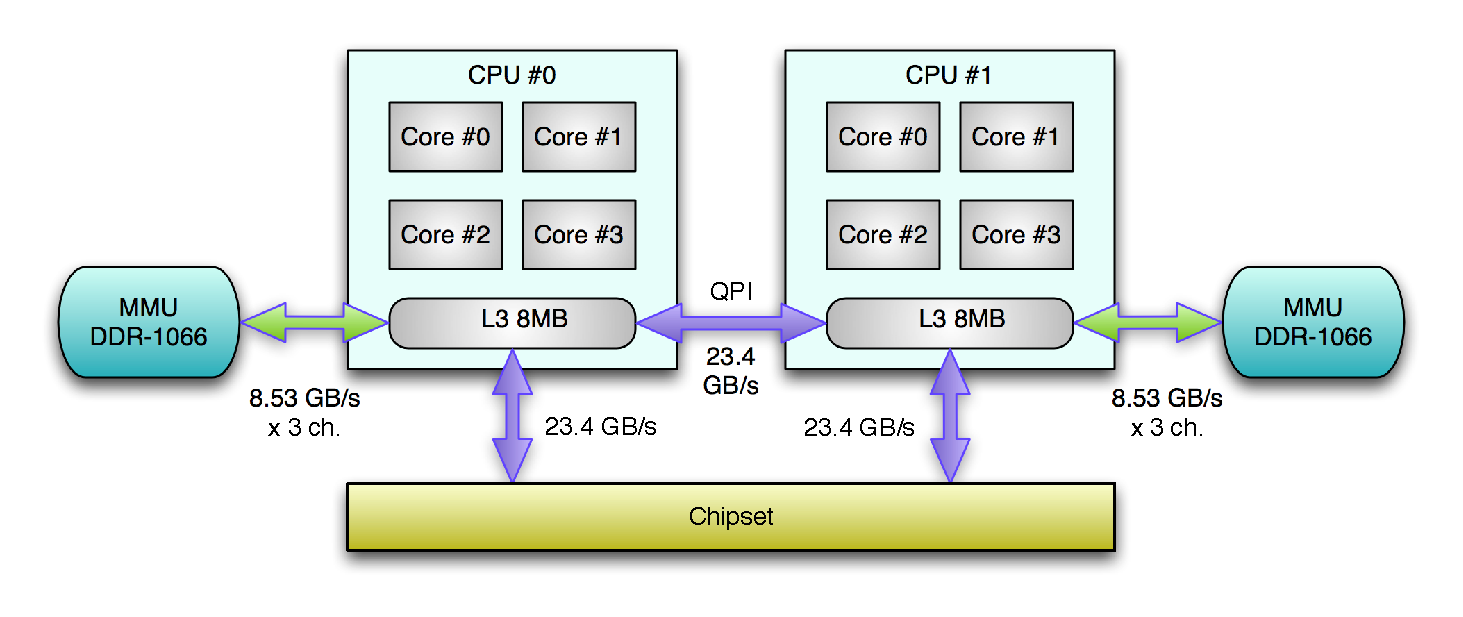
\includegraphics[width=14cm,clip]{E5520_arch.eps}
\end{center}
\caption{E5520のアーキテクチャー}
\label{fig:nehalem}
\end{figure}

QPIはQuickPath Interconnectで高速シリアルP2Pインターコネクトで,1リンク(片方向)あたり20bit(16bit-data, 2bit-protocol, 2bit-CRC error check)である\footnote{QPIはI/Oインターフェースではなく,システムはPCI-EをI/Oに利用する.}.
E5520のQPIは1リンクあたり5.86GT/sで,2リンク(双方向)時23.44GB/s$(=5.86\times 2B \times 2)$となる.
メモリバンド幅はDDR-1066(8.53GB/s)の3チャネルで,CPUあたり25.6GB/sとなる.

Nehalemコアの理論最大性能は1cycleあたり4浮動小数点演算が可能で,packed SSE(SIMD)命令により加算器と乗算器が同時に動作する場合にのみ達成される.
したがって,\hyperlink{tgt:perf prediction}{性能評価}で参照するCPUあたりのマシンバランス$B_M$は以下のようになる.

\begin{equation}
B_M \,=\, \frac{8.53\,GB/s \times 3\,ch.}{(4\,FLOP/cycle \times 2.26\,GHz) \times 4\,core} \,=\, \frac{25.6\,GB/s}{36.16\,GFLOPS} \sim 0.7\,B/F
\label{eq:B_M nehalem}
\end{equation}



%
\subsection{MacPro - Westmere}

MacPro(Westmere)の諸元を\textbf{表\ref{tbl:macpro-westmere}}に示す\footnote{\url{http://ark.intel.com/Product.aspx?id=47922}}.

\begin{table}[htdp]
\caption{Specification of MacPro(Westmere)}
\small
\begin{center}
\begin{tabular}{rl} \toprule
Processor & Intel Xeon X5650\\
\# of core & 6\\
\# of CPU & 2\\
Clock & 2.66 GHz\\
2nd cache & 256 kB (each core)\\
3rd cache & 12 MB (each proc.)\\
Peak FP rate Multi+Add & 4 flop/cycle\\
QPI speed & 6.4 GT/s (=25.6 GB/s)\\
Memory & DDR3-1333 (3ch.)\\ \bottomrule
\end{tabular}
\end{center}
\label{tbl:macpro-westmere}
\end{table}


\textbf{図\ref{fig:westmere}}にX5650プロセッサのアーキテクチャーを示す.

\begin{figure}[htdp]
\begin{center}
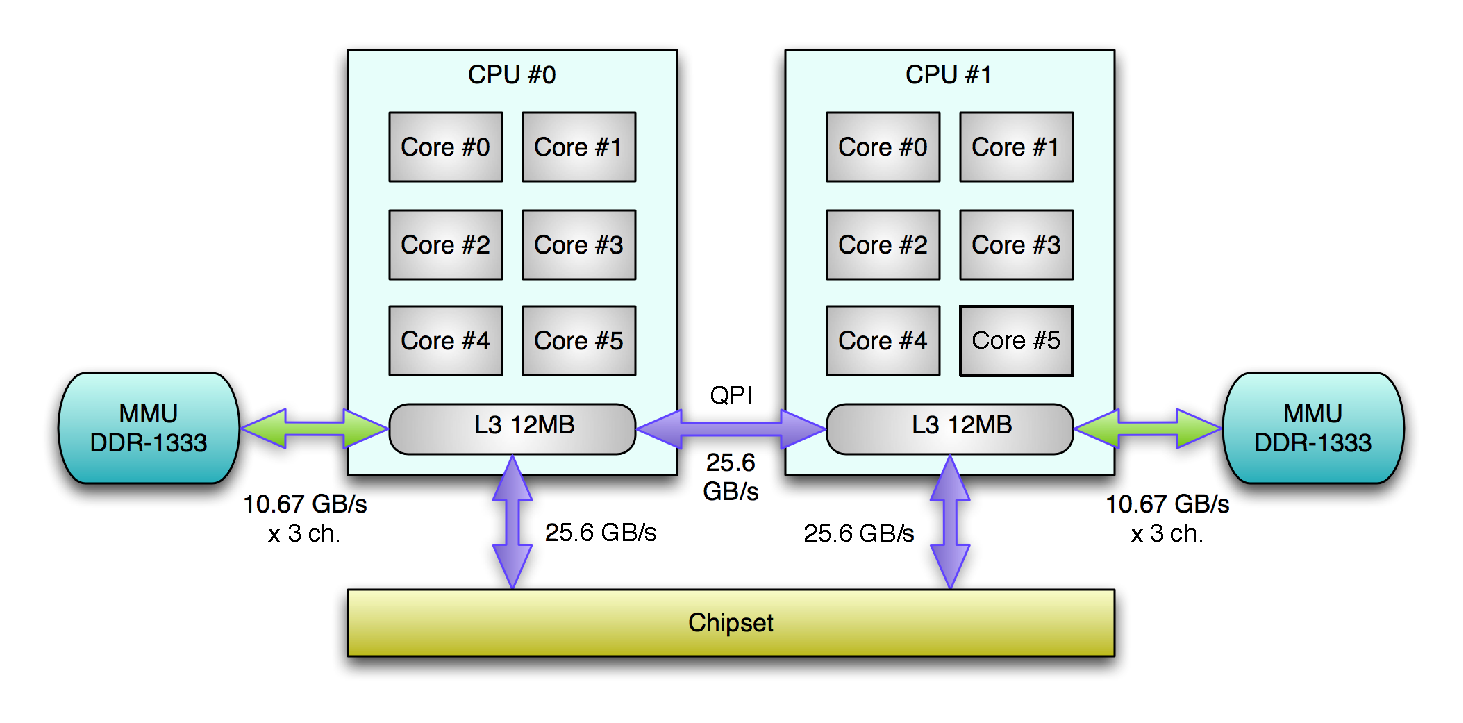
\includegraphics[width=14cm,clip]{X5650_arch.eps}
\end{center}
\caption{X5650のアーキテクチャー}
\label{fig:westmere}
\end{figure}

E5520と異なり,QPIは1リンクあたり6.4GT/sなので,双方向時にはQPI最大性能の25.6GB/sとなる.
また,メモリバンド幅はDDR-1333(10.67GB/s)なのでCPUあたり32GB/sである.
したがって,CPUあたりのマシンバランス$B_M$は以下のようになる.
NehalemよりもWestmereの方がByte/Flopは小さく,sustainedな計算には不利である.

\begin{equation}
B_M \,=\, \frac{10.67\,GB/s \times 3\,ch.}{(4\,FLOP/cycle \times 2.66\,GHz) \times 6\,core} \,=\, \frac{32.0\,GB/s}{63.84\,GFLOPS} \sim 0.5\,B/F
\label{eq:B_M westmere}
\end{equation}




%
\subsection{RICC}

RICC(Riken Integrated Cluster of Clusters)~\cite{ricc}の諸元を\textbf{表\ref{tbl:ricc}}に示す.
ネットワークにInfiniband x4 DDR\footnote{IB DDRは5Gbpsでデータ幅は8/10bitなので実質的に4Gbps=0.5GB/s.x4はその4倍で2GB/s.}を用いており,aggregate performanceは2TB/s,Bisection Bandwidthは240GB/sである.

\begin{table}[htdp]
\caption{Specification of RICC}
\small
\begin{center}
\begin{tabular}{rl}\toprule
Processor & Intel Xeon X5570\\
\# of core & 4\\
\# of CPU & 2\\
\# of Node & 1024\\
Clock & 2.93 GHz\\
2nd cache & 256 kB (each core)\\
3rd cache & 8 MB (each proc.)\\
Peak FP rate Multi+Add & 4 flop/cycle\\
QPI speed & 6.4 GT/s (=25.6 GB/s)\\
Memory & DDR3-1333 (3ch.)\\
Interconnect & IB x4 DDR (=2 GB/s)\\
Bisection bandwidth & 240 GB/s\\ \bottomrule
\end{tabular}
\end{center}
\label{tbl:ricc}
\end{table}


\begin{equation}
B_M \,=\, \frac{10.67\,GB/s \times 3\,ch.}{(4\,FLOP/cycle \times 2.93\,GHz) \times 4\,core} \,=\, \frac{32.0\,GB/s}{46.88\,GFLOPS} \sim 0.68\,B/F
\label{eq:B_M ricc}
\end{equation}

%
\subsection{FOCUS}
FOCUS~\cite{focus}の諸元を\textbf{表\ref{tbl:focus}}に示す.
バイセクションバンド幅は,x4 DDR双方向で$208nodes/2 \times 2GB/s \times 2\,=\,416\,GB/s$である.

\begin{table}[htdp]
\caption{Specification of FOCUS}
\small
\begin{center}
\begin{tabular}{rl}\toprule
Processor & Intel Xeon L5640\\
\# of core & 6\\
\# of CPU & 2\\
\# of Node & 208\\
Clock & 2.26 GHz\\
2nd cache & 256 kB (each core)\\
3rd cache & 12 MB (each proc.)\\
Peak FP rate Multi+Add & 4 flop/cycle\\
QPI speed & 5.86 GT/s (=23.44 GB/s)\\
Memory & DDR3-1333 (3ch.)\\
Interconnect & IB x4 DDR (=2 GB/s)\\
Bisection bandwidth & 416 GB/s\\ \bottomrule
\end{tabular}
\end{center}
\label{tbl:focus}
\end{table}

\begin{equation}
B_M \,=\, \frac{10.67\,GB/s \times 3\,ch.}{(4\,FLOP/cycle \times 2.26\,GHz) \times 6\,core} \,=\, \frac{32.0\,GB/s}{54.24\,GFLOPS} \sim 0.59\,B/F
\label{eq:B_M focus}
\end{equation}

%
%\subsection{K}

\pagebreak

%%
\section{FlatMPIの性能測定結果}
CBCソルバークラスの実効性能を各計算機上で測定した.
並列実行はFlatMPIである.

%
\subsection{MacPro - Nehalem}
\textbf{表\ref{tbl:macpro-env-nehalem}}に実行環境とシステム性能を示す.
\textbf{図\ref{fig:mac-nehalem-perf}}から8コア時の性能は14.4GFLOPSなので,理論性能の20\%の実行性能である.

\begin{table}[htdp]
\caption{Execution environment of MacPro(Nehalem)}
\small
\begin{center}
\begin{tabular}{rl}\toprule
System peak performance & 72.3 GFLOPS\\
Compiler & Intel C/C++, Fortran 12.0.2.142\\
Compiler option & -O3\\
MPI library & OpenMPI 1.4.1\\
V-Sphere & 1.8.3\\
CBC & 1.3.1\\
FB & 2.3.3\\
OS & 10.6.7 (Darwin 10.7.0)\\
Date of measurement & 2010-12-16\\ \bottomrule
\end{tabular}
\end{center}
\label{tbl:macpro-env-nehalem}
\end{table}

\begin{figure}[htdp]
\begin{center}
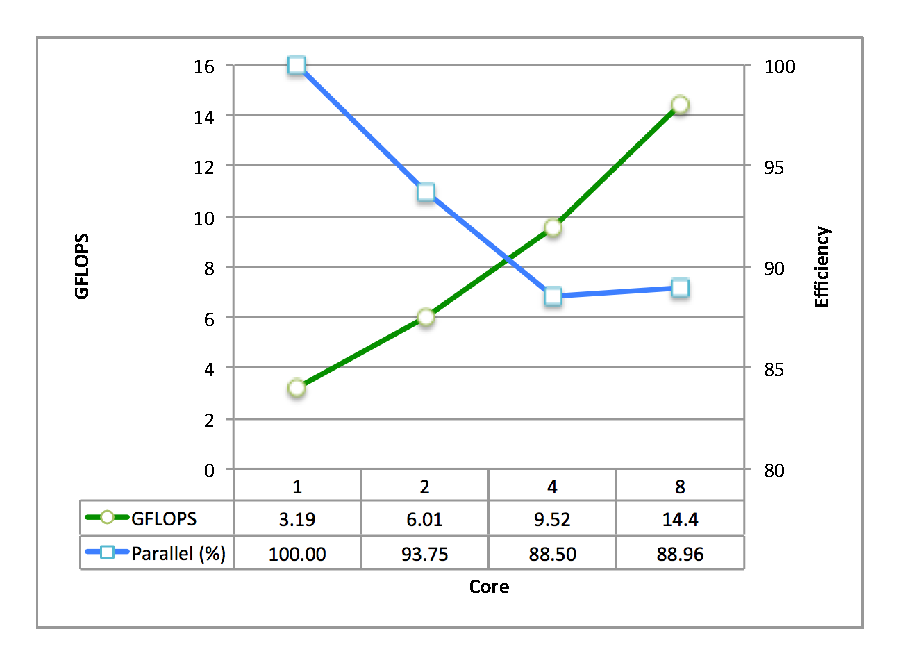
\includegraphics[height=8cm,clip]{mac-nehalem.eps}
\end{center}
\caption{MacPro(Nehalem)での実行性能}
\label{fig:mac-nehalem-perf}
\end{figure}

\pagebreak
%
\subsection{MacPro - Westmere}

\textbf{表\ref{tbl:macpro-env-westmere}}に実行環境とシステム性能を示す.
\textbf{図\ref{fig:mac-westmere-perf}}から12コア時の性能は18.6GFLOPSなので,理論性能の14.6\%の実行性能である.

Nehalemの場合も同様であるが,コア数が増える場合の並列性能の落ち込みは,MMU-CPU間のバンド幅におけるデータ供給量の飽和による.
CBCソルバークラスは,データ供給によって実効性能が制限される特性をもつ(Memory Bound).
マルチコア環境でアフィニティ制御を行わないと,プロセスはCPUのコアに詰めて割り振られる(デフォルトのポリシー).
この場合,CPU内で動いているコア数だけメモリへデータのダウンロード要求を出すのでメモリバンド幅は飽和し,相対的にデータ供給が低下し,性能劣化を引き起こす.
メモリへのデータの割り付けとコアのマッピングは制御していないので,場合によってはコアがリモートのメモリへアクセスすることもある.
その場合にはQPI経由になるので,データ転送速度はさらに低下する可能性がある.

\begin{table}[htdp]
\caption{Execution environment of MacPro(Westmere)}
\small
\begin{center}
\begin{tabular}{rl}\toprule
System peak performance & 127.7 GFLOPS\\
Compiler & Intel C/C++, Fortran 12.0.3.167\\
Compiler option & -O3\\
MPI library & OpenMPI 1.4.3\\
V-Sphere & 1.8.4\\
CBC & 1.3.5\\
FB & 2.3.6\\
OS & 10.6.8 (Darwin 10.8.0)\\
Date of measurement & 2011-06-28\\ \bottomrule
\end{tabular}
\end{center}
\label{tbl:macpro-env-westmere}
\end{table}

\begin{figure}[htdp]
\begin{center}
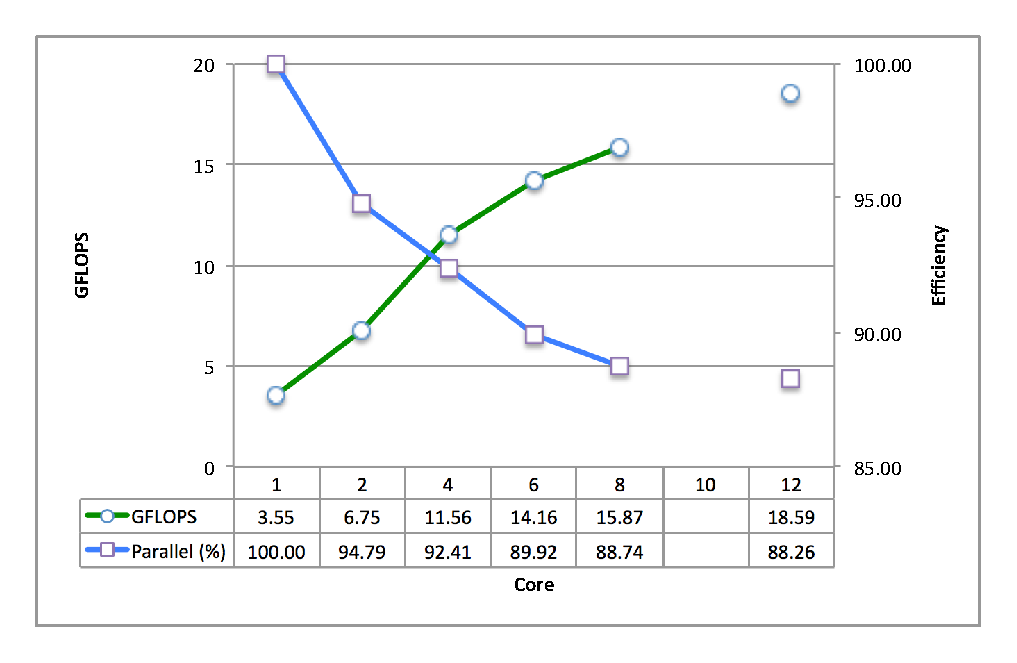
\includegraphics[height=8cm,clip]{mac-westmere.eps}
\end{center}
\caption{MacPro(Westmere)での実行性能}
\label{fig:mac-westmere-perf}
\end{figure}

\pagebreak
%
\subsection{RICC}

\textbf{表\ref{tbl:ricc-env}}にRICCの実行環境とシステム性能を示す.
\textbf{図\ref{fig:ricc-perf}}から8192コア時の性能は10TFLOPSなので,理論性能の10.4\%の実行性能である.


コア数が少ないところでの並列性能の落ち込みは,上述したようにノード内の帯域の問題である.
影響の現れ方は,コアへのプロセスマッピングポリシーに依存する.
各ノード内のコアが全て使われた状態でノード数が増加しているので,良好なスケーラビリティを見せている.

\begin{table}[htdp]
\caption{Execution environment of RICC}
\small
\begin{center}
\begin{tabular}{rl}\toprule
System peak performance & 96 TFLOPS\\
Compiler & Intel C/C++, Fortran 11.1.073\\
Compiler option & -O3\\
MPI library & OpenMPI 1.4.0?\\
V-Sphere & 1.8.3\\
CBC & 1.3.1\\
FB & 2.3.3\\
OS & RedHat\\
Date of measurement & 2011-02-28\\ \bottomrule
\end{tabular}
\end{center}
\label{tbl:ricc-env}
\end{table}

\begin{figure}[htdp]
\begin{center}
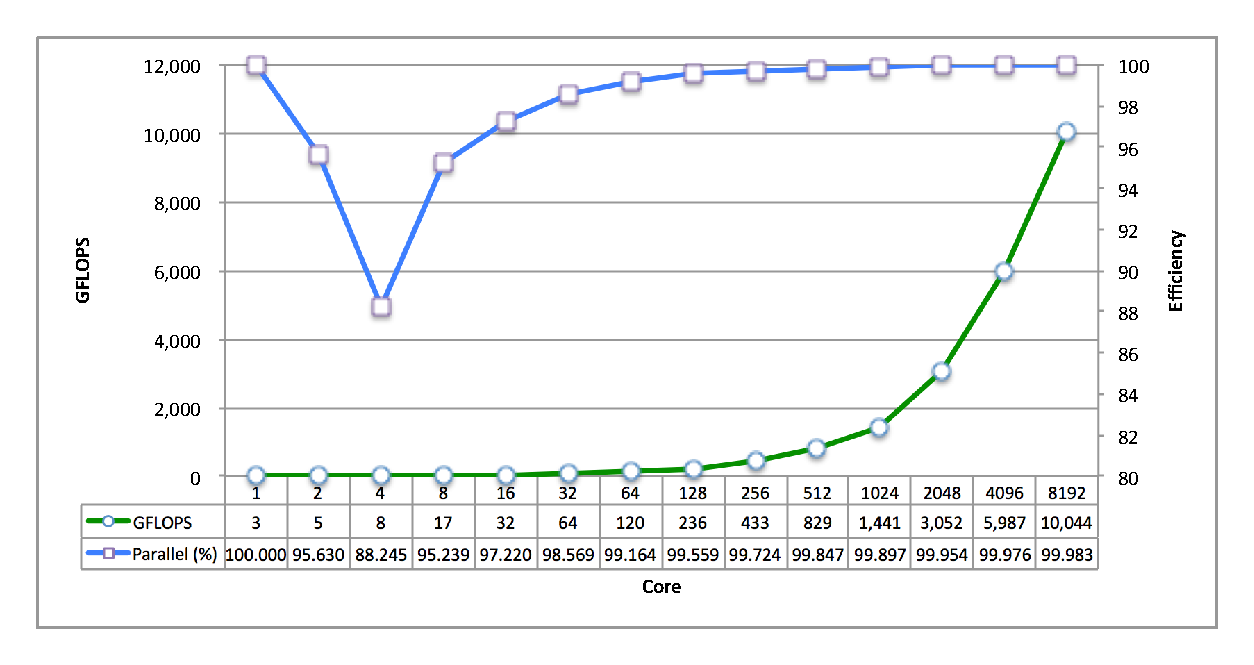
\includegraphics[height=8cm,clip]{ricc.eps}
\end{center}
\caption{RICCでの実行性能}
\label{fig:ricc-perf}
\end{figure}

\pagebreak
%
\subsection{FOCUS}

\textbf{表\ref{tbl:focus-env}}にRICCの実行環境とシステム性能を示す.
利用できるコア数は64ノード(768コア)なので,その場合のシステム性能は6943GFLOPSである.
\textbf{図\ref{fig:focus-perf}}から768コア時の性能は1036GFLOPSなので,理論性能の14.9\%の実行性能である.

\begin{table}[htdp]
\caption{Execution environment of FOCUS}
\small
\begin{center}
\begin{tabular}{rl}\toprule
System peak performance & 22.6 TFLOPS / 208nodes (6942.7 GFLOPS / 64 nodes)\\
Compiler & Intel C/C++, Fortran 12.0.084\\
Compiler option & -O3\\
MPI library & OpenMPI 1.4.1\\
V-Sphere & 1.8.4\\
CBC & 1.3.1\\
FB & 2.3.3\\
OS & Cent OS, Linux Kernel 2.6\\
Date of measurement & 2011-04-08\\ \bottomrule
\end{tabular}
\end{center}
\label{tbl:focus-env}
\end{table}

\begin{figure}[htdp]
\begin{center}
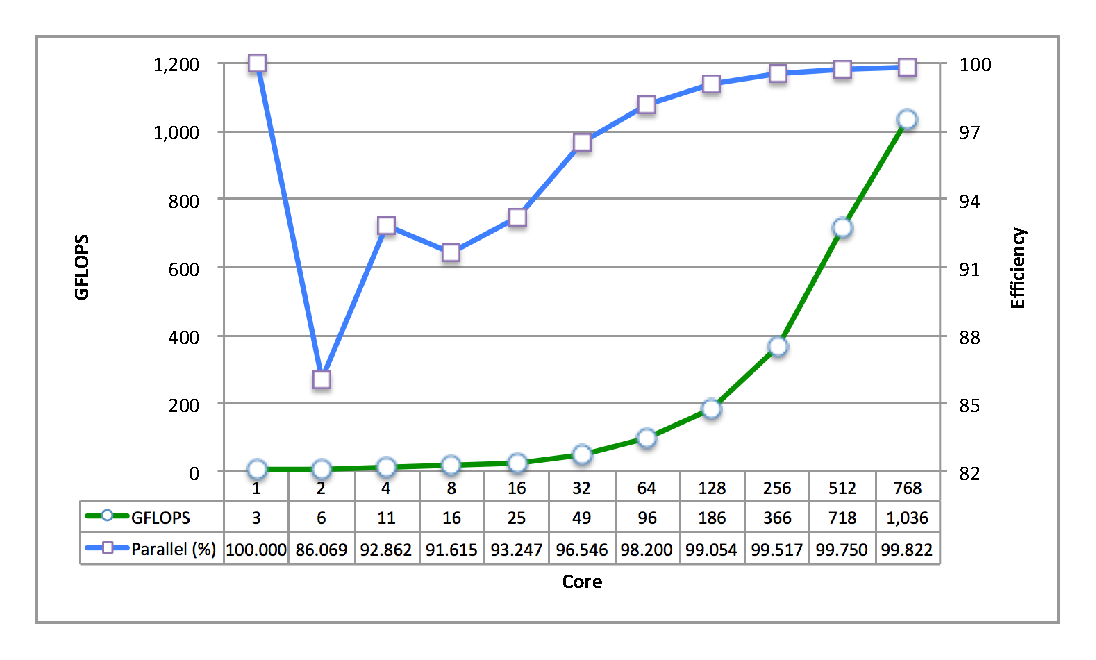
\includegraphics[height=8cm,clip]{focus.eps}
\end{center}
\caption{FOCUSでの実行性能}
\label{fig:focus-perf}
\end{figure}

\pagebreak
%%
\hypertarget{tgt:perf prediction}{\section{性能評価}}
%
\subsection{Machine Balance}



た\cite{treibig:10:springerlink}
